\graphicspath{{6residues/asy/}}

\section{Laurent Series, Residues and Poles}\label{chap:residue}


While Taylor series are undeniably useful, they also have weaknesses, not least because their domains are \emph{disks.} We motivate a more general construction with an example.

\begin{example}{}{laurentmotiv}
	$f(z)=\frac 1{z(2-z)}$ can be written as a Taylor series centered at $z=1$:\par
	\begin{minipage}[t]{0.7\linewidth}\vspace{-10pt}
		\[
			f(z)=\frac 1{1-(z-1)^2} 
			=\sum_{n=0}^\infty (z-1)^{2n}
			\quad\text{whenever \ \textcolor{Green}{$\nm{z-1}<1$}}
		\]
		However, we are also interested in the behavior of $f(z)$ near the points $z=0,2$. Due to their disk-domains, we can't use Taylor series to loop around these points.\smallbreak
		As an alternative, start with the Maclaurin series for $\frac 1{2-z}$ (valid when $\nm z<2$) and divide through by $z$ to obtain a new expression:
	\end{minipage}
	\hfill
	\begin{minipage}[t]{0.29\linewidth}\vspace{-10pt}
		\flushright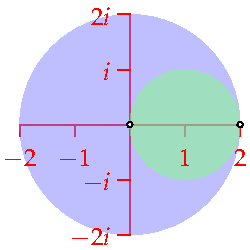
\includegraphics[scale=0.95]{laurent}
	\end{minipage}\par\vspace{-2pt}
	\[
		f(z)=\frac 1{2z(1-\frac{z}{2})}
		=\frac 1{2z}\sum_{n=0}^\infty\left(\frac z2\right)^n 
		=\sum_{n=-1}^\infty\frac{z^n}{2^{n+2}} =\frac 1{2z}+\frac 14+\frac z8+\frac{z^2}{16}+\frac{z^3}{32}+\cdots	
	\]
	By construction, this `series with negative terms' is valid on the \textcolor{blue}{punctured disk $0<\nm z<2$}.
\end{example}

\subsection{Laurent Series}\label{sec:laurent}

Series with negative terms are very useful in complex analysis. In Example \ref{ex:laurentmotiv}, the larger domain encircling the origin provides an obvious advantage over the Taylor series. That such a series converges on an \textcolor{blue}{annulus} rather than a disk is typical. We omit the full details, but by splitting a general series into positive and negative powers, substituting $w=(z-z_0)^{-1}$, and applying Theorems \ref{thm:absconv}, \ref{thm:unifconv} and \ref{thm:seriescont} to the resulting power series in $w$
\[
	\sum\limits_{n=-\infty}^{\infty} a_n(z-z_0)^n=\sum\limits_{n=0}^{\infty} a_n(z-z_0)^n+\sum\limits_{n=-\infty}^{-1} a_n(z-z_0)^n
	=\sum\limits_{n=0}^{\infty} a_n(z-z_0)^n +\sum\limits_{n=1}^\infty a_{-n}w^n
\]
one obtains the natural extensions of these results.

\begin{thm}{Annulus of convergence}{}
	Given a series $\smash[b]{\sum\limits_{n=-\infty}^{\smash{\infty}} a_n(z-z_0)^n}$, define\par
	\begin{minipage}[t]{0.7\linewidth}\vspace{-14pt}
		\begin{gather*}
			\textcolor{Magenta}{R_1}=\inf\bigl\{\nm{z-z_0}:f(z)\text{ converges}\bigr\}\\
			\textcolor{red}{R_2}=\sup\bigl\{\nm{z-z_0}:f(z)\text{ converges}\bigr\}
		\end{gather*}
		\begin{enumerate}
		  \item The series converges absolutely to a continuous function on the (open) \emph{\textcolor{blue}{annulus of convergence}} $R_1<\nm{z-z_0}<R_2$. The convergence is moreover uniform on any closed sub-annulus.
		  \item If \textcolor{Magenta}{$\nm{z-z_0}<R_1$} or \textcolor{red}{$\nm{z-z_0}>R_2$}, the series diverges.
		\end{enumerate}
	\end{minipage}
	\hfill
	\begin{minipage}[t]{0.29\linewidth}\vspace{0pt}
		\hfill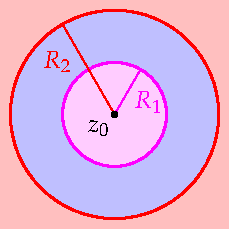
\includegraphics[scale=0.95]{laurent8}
	\end{minipage}\medbreak
	As with power series, convergence on the \textcolor{Magenta}{boundary} \textcolor{red}{circles} must be checked separately.
\end{thm}

As in Example \ref{ex:laurentmotiv}, the inner radius can be $R_1=0$ and the domain a punctured disk. Moreover, the outer radius can be $R_2=\infty$.\smallbreak

\goodbreak

As with Taylor series, our goal is often to find a series representation of a given function.

\begin{defn}[lower separated=false, sidebyside, sidebyside align=top seam, sidebyside gap=0pt, righthand width=0.25\linewidth]{}{laurent}
	Suppose $f(z)$ is analytic on an \textcolor{Green}{\emph{annulus}} $R_1<\nm{z-z_0}<R_2$. Its \emph{Laurent series} centered at $z_0$ is the expression
	\[
		\sum_{n=-\infty}^\infty a_n(z-z_0)^n
		\ \text{ where }\ 
		a_n=\frac 1{2\pi i}\oint_C\frac{f(z)}{(z-z_0)^{n+1}}\,\dz
	\]
	and \textcolor{red}{$C$} is any simple closed contour encircling $z_0$ within the annulus.
	\tcblower
	\flushright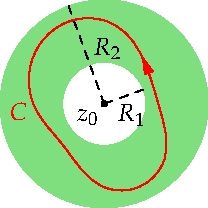
\includegraphics[scale=0.95]{laurent2}
\end{defn}

\begin{itemize}
  \item If you prefer, write $\sum\limits_{n=0}^\infty a_n(z-z_0)^n+\sum\limits_{n=1}^\infty \frac{b_n}{(z-z_0)^n}$ where $b_n=\frac 1{2\pi i}\oint_C(z-z_0)^{n-1}f(z)\,\dz$.\par
  \begin{minipage}[t]{0.73\linewidth}\vspace{0pt}
		\item The coefficients $a_n$ are independent of the choice of contour $C$.\smallbreak
		To see this, suppose $D$ is another simple closed curve encircling $z_0$, and choose a circle $E$ outside both $C$ and $D$. Since $\frac{f(z)}{(z-z_0)^{n+1}}$ is analytic on the annulus, two applications of Cauchy--Goursat yield
	  \[
	  	\oint_{\textcolor{red}{C}}\frac{f(z)}{(z-z_0)^{n+1}}\,\dz
	  	=\oint_{\textcolor{purple}{E}}\frac{f(z)}{(z-z_0)^{n+1}}\,\dz
	  	=\oint_{\textcolor{blue}{D}}\frac{f(z)}{(z-z_0)^{n+1}}\,\dz
	  \]
	\end{minipage}
	\hfill
	\begin{minipage}[t]{0.26\linewidth}\vspace{-5pt}
		\flushright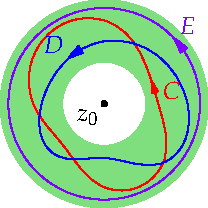
\includegraphics[scale=0.95]{laurent3}
	\end{minipage}\par
  
  \item The Laurent coefficients are inspired by our discussion of Taylor series. If $f(z)$ happens to be analytic on the \emph{disk} $\nm{z-z_0}<R_2$, then its Laurent series equals the Taylor series:
	\[
		\begin{cases}
			n\ge 0\implies a_n=\frac{f^{(n)}(z_0)}{n!} \quad &\text{(Cauchy's integral formula)}\\
			n<0\implies a_n=0 \quad &\text{(Cauchy--Goursat)}
		\end{cases}
	\]
	Typically, however, $f(z)$ is not defined (or analytic) at $z_0$. Laurent series therefore generalize and replace Taylor series in such situations.
\end{itemize}

\begin{example*}{\ref{ex:laurentmotiv}, cont.}{}
	$f(z)=\frac 1{z(2-z)}$ is certainly analytic on the \textcolor{blue}{annulus} $0<\nm z<2$.\par
	\begin{minipage}[t]{0.7\linewidth}\vspace{-4pt}
		By first writing $f(z)=\frac 12\left(\frac 1{z}+\frac 1{2-z}\right)$ using partial fractions, we compute the Laurent series for $f$ on the annulus using the \textcolor{Green}{unit circle} centered at the origin:
		\[
			a_n=\frac 1{2\pi i}\oint_C\frac{f(z)}{z^{n+1}}\,\dz =\frac 1{4\pi i}\oint_C \frac{1}{z^{n+2}}+\frac 1{(2-z)z^{n+1}}\,\dz
		\]
		The first integral evaluates to $\frac 12$ when $n=-1$ and to zero otherwise. The second  integral may be found using Cauchy's integral formula:
	\end{minipage}
	\hfill
	\begin{minipage}[t]{0.29\linewidth}\vspace{-4pt}
		\flushright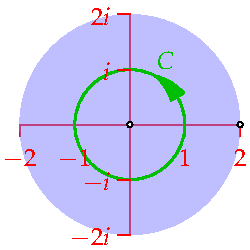
\includegraphics[scale=0.95]{laurent7}
	\end{minipage}\par
	\[
		\frac 1{4\pi i}\oint_C \frac 1{(2-z)z^{n+1}}\,\dz =
		\begin{cases}
			0&\text{if }n\le -1\\
			\displaystyle\frac 1{2(n!)}\diffat[{}^n]{z^n}{z=0}(2-z)^{-1} =\frac 1{2^{n+2}}&\text{if }n\ge 0
		\end{cases}
	\]
	We conclude that $a_n=\frac 1{2^{n+2}}$: the Laurent series of $f(z)$ is precisely the series computed previously!\smallbreak
	The Laurent series centered at $z_0=2$ can be computed similarly, both using the integral method and our original approach. 
\end{example*}

The example is typical. Computing a Laurent series directly from the definition is usually ugly given how many contour integrals must be evaluated! Thankfully, as we'll see shortly, all the standard facts regarding Taylor series translate to this new situation. In particular, if $f(z)=\sum a_n(z-z_0)^n$ equals a series with negative terms, then the series will turn out to be the Laurent series of $f(z)$. We'll deal with the theory shortly, but first a few more examples following from this observation to get used to the idea.



\begin{examples}{}{laurenteasyex}
	\exstart On the \textcolor{blue}{disk $\nm z<1$}, we have the Maclaurin series
	
	\begin{enumerate}\setcounter{enumi}{1}
	  \begin{minipage}[t]{0.73\linewidth}\vspace{-13pt}
		  \item[]%
		  \[
		  	\frac 1{z-i}=\frac 1{-i(1-\frac zi)}
		  	=i\sum_{n=0}^\infty(-iz)^n
		  	=i+z-iz^2-z^3+iz^4+\cdots
		  \]
			On the \textcolor{Green}{annulus $\nm z>1$}, we have the Laurent series
			\[
				\frac 1{z-i}=\frac z{(1-\frac iz)}
				=\sum_{n=0}^\infty i^nz^{-n-1}
				=\frac iz-\frac 1{z^2}-\frac i{z^3}+\frac 1{z^4}+\cdots
			\]
		
			\item On the \textcolor{orange}{$1<\nm z<2$}, we have the Laurent series
			\begin{align*}
				\frac 3{(2-z)(1+z)}
				&=\frac 1{2-z}+\frac 1{1+z}=\frac 1{2(1-\frac z2)}+\frac 1{z(1+\frac 1z)} \\
				&=\frac 12\sum_{n=0}^\infty\left(\frac z2\right)^n+\frac 1z\sum_{m=0}^\infty(-z)^{-m}\\
				&=\cdots +z^{-3}-z^{-2}+z^{-1}+\frac 12+\frac 14z+\frac 18z^2+\cdots
			\end{align*}
		\end{minipage}
		\hfill
		\begin{minipage}[t]{0.26\linewidth}\vspace{-20pt}
			\flushright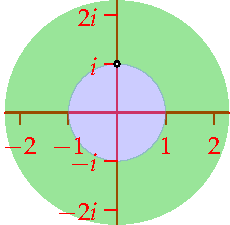
\includegraphics[scale=0.95]{laurent5}\bigbreak
			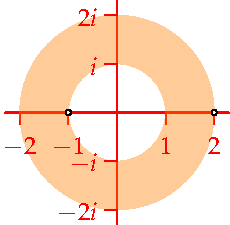
\includegraphics[scale=0.95]{laurent6}
		\end{minipage}\par	
		
	
	  \item Since $e^z=\sum \frac{z^n}{n!}$ is valid on the entire complex plane, we obtain the Laurent series expansion
	  \[
	  	e^{\frac 1z}=\sum_{n=0}^\infty\frac{z^{-n}}{n!}=1+\frac 1z+\frac 1{2z^2}+\frac 1{6z^3}+\cdots
	  \]
	  valid on the punctured plane $z\neq 0$.
	  
	  \item Again by substituting in a known Maclaurin series, we obtain another Laurent series valid on the punctured plane $z\neq 0$:
	  \[
	  	\frac 1{z^7}\sin z^2
	  	=\sum_{n=0}^\infty\frac{(-1)^n}{(2n+1)!}z^{4n-5} 
	  	=z^{-5}-\frac 16z^{-1}+\frac 1{120}z^3-\frac 1{5040}z^7+\cdots
	  \]
	  
	  \item Multiplying term-by-term, and since we need \emph{both} Maclaurin series to be valid, we obtain (the first few terms of) a Laurent series valid on the punctured disk $0<\nm z<1$:
	  \begin{align*}
		  \frac 1{z(z-1)(z-2i)}&=\frac 1z\left(\sum_{n=0}^\infty (-1)^nz^n\right)\left(\sum_{m=0}^\infty\left(\frac i2\right)^mz^m\right)\\
		  &=\frac 1z\left(1-z+z^2-z^3+\cdots\right)\left(1+\frac i2z-\frac 14z^2-\frac i8z^3+\cdots\right)\\
		  &=\frac 1z+\left(-1+\frac i2\right)+\left(\frac 34-\frac i2\right)z+\left(-\frac 34+\frac{3i}8\right)z^2+\cdots
	  \end{align*}
	\end{enumerate}
\end{examples}

\goodbreak


%\boldsubsubsection{Theory time!}

We now state and prove the main properties of Laurent series. These are very similar to the corresponding statements \& arguments for Taylor series; the additional challenge mostly comes from keeping track of two series at once.

\begin{thm}{Laurent's Theorem}{laurent}
	An analytic function on an open annulus equals its Laurent series.
\end{thm}

\begin{proof}
	It is enough to prove when the annulus is centered at $z_0=0$. Let $w$ in the annulus be given.\par
	\begin{minipage}[t]{0.73\linewidth}\vspace{-3pt}
		Since the annulus is open, we may choose three non-overlapping circles $\alpha,\beta,\gamma$ with radii $R_\alpha,R_\beta,R_\gamma$ as in the picture:
		\begin{itemize}
		  \item $\gamma$ a \textcolor{Green}{small circle} centered at $w$ inside the annulus;
		  \item $\alpha,\beta$ centered at 0, \textcolor{red}{$\alpha$ inside} and \textcolor{orange}{$\beta$ outside} $w$ (thus $R_\alpha<\nm w<R_\beta$). 
		\end{itemize}
		Since $\frac{f(z)}{z-w}$ is analytic on/inside the closed region with boundaries $\alpha,\beta,\gamma$, Cauchy--Goursat and the integral formula tell us that
	\end{minipage}
	\hfill
	\begin{minipage}[t]{0.25\linewidth}\vspace{-4pt}
		\flushright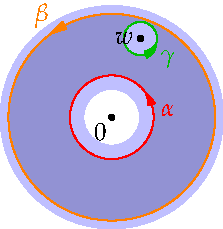
\includegraphics[scale=0.95]{laurent4}
	\end{minipage}\par
	\[
		\left(\oint_\beta-\oint_\alpha-\oint_\gamma\right)\frac{f(z)}{z-w}\,\dz=0\implies f(w)=\frac 1{2\pi i}\oint_\gamma\frac{f(z)}{z-w}\,\dz =\frac 1{2\pi i}\left(\oint_\beta-\oint_\alpha\right)\frac{f(z)}{z-w}\,\dz
		\tag{$\ast$}
	\]
	As in the proof of Taylor's theorem, we expand $\frac 1{z-w}$, this time in two ways:
	\[
		\frac 1{z-w}
		=\frac 1z\sum_{k=0}^{n-1}\left(\frac wz\right)^k +\frac 1{z-w}\left(\frac wz\right)^n 
		=-\frac 1w\sum_{k=1}^{n}\left(\frac zw\right)^{k-1} +\frac 1{z-w}\left(\frac zw\right)^n
	\]
	These expansions allow us to attack the two integrals in ($\ast$):
	\begin{gather*}
		\frac 1{2\pi i}\oint_\beta\frac{f(z)}{z-w}\,\dz
		=\sum_{k=0}^{n-1}\underbrace{\frac{w^k}{2\pi i}\oint_\beta \frac{f(z)}{z^{k+1}}\,\dz}_{a_kw^k} +\frac{w^n}{2\pi i}\oint_\beta \frac{f(z)}{z^n(z-w)}\,\dz\\
		\frac{-1}{2\pi i}\oint_\alpha\frac{f(z)}{z-w}\,\dz =\sum_{k=1}^{n}\underbrace{\frac 1{2\pi iw^k}\oint_\alpha z^{k-1}f(z)\,\dz}_{a_{-k}w^{-k}} -\frac 1{2\pi i w^n}\oint_\alpha \frac{z^nf(z)}{z-w}\,\dz
	\end{gather*}
	We finish by summing and estimating, using the facts that $z\in\alpha\cup\beta\Longrightarrow\nm{z-w}>R_\gamma$, and that $f(z)$ is bounded (by some $M>0$) on the closed bounded annulus between $\alpha,\beta$:
	\begin{align*}
		\nm{f(w)-\sum_{k=-n}^{n-1}a_kw^k}
		&=\nm{\frac{w^n}{2\pi i}\oint_\beta \frac{f(z)}{z^n(z-w)}\,\dz -\frac 1{2\pi iw^n}\oint_\alpha \frac{z^nf(z)}{z-w}\,\dz}\\
		&\overset{\triangle}{\le} \frac{\nm w^n}{2\pi}\nm{\oint_\beta \frac{f(z)}{z^n(z-w)}\,\dz} +\frac 1{2\pi\nm w^n}\nm{\oint_\alpha \frac{z^nf(z)}{z-w}\,\dz}\\
		&\le \frac{\nm w^n}{2\pi}\cdot\frac{M}{R_\beta^nR_\gamma}\cdot 2\pi R_\beta +\frac 1{2\pi\nm w^n}\cdot \frac{R_\alpha^nM}{R_\gamma}\cdot 2\pi R_\alpha
			\tag{Theorem \ref{thm:intbound}}\\
		&=\frac M{R_\gamma}\left[R_\beta\left(\frac{\nm w}{R_\beta}\right)^n+R_\alpha\left(\frac{R_\alpha}{\nm w}\right)^n\right] \xrightarrow[n\to\infty]{} 0
		\tag*{\qedhere}
	\end{align*}
\end{proof}

\goodbreak


% \begin{defn}{}{}
% 	Given a series $\smash[b]{f(z)=\sum\limits_{n=-\infty}^\infty a_n(z-z_0)^n}$, define
% 	\[
% 		R_1=\inf\bigl\{\nm{z-z_0}:f(z)\text{ converges}\bigr\},\qquad 
% 		R_2=\sup\bigl\{\nm{z-z_0}:f(z)\text{ converges}\bigr\}
% 	\]
% 	The region $R_1<\nm{z-z_0}<R_2$ is called the (open) \emph{annulus of convergence.}
% \end{defn}

Our final corollary summarizes the remaining core properties of Laurent series.


\begin{cor}{}{laurenttidy}
	Let $f(z)=\sum a_n(z-z_0)^n$ be a series. Then:
	\begin{enumerate}
% 	  \item On its open annulus of convergence, $f(z)$ converges absolutely to a continuous function. As with power series, convergence on the boundary circles must be checked separately.
% 	  \item The convergence is uniform on any closed sub-annulus.
  	\item\label{cor:laurtidy3} (Term-by-term Integration)\quad If $g(z)$ is continuous on a contour $C$ lying inside the annulus, then
  	\[
  		\int_C g(z)f(z)\,\dz=\sum_{n=-\infty}^\infty a_n\int_Cg(z)(z-z_0)^n\,\dz
  	\]
  	In particular, $f(z)$ may be integrated term-by-term along $C$.
 
 		\item\label{cor:laurtidy4} (Analyticity/Derivatives)\quad $f(z)$ is analytic on the annulus and $f'(z)=\sum\limits_{n=-\infty}^\infty a_nn(z-z_0)^{n-1}$
  	
  	\item\label{cor:laurtidy5} (Uniqueness)\quad $\sum a_n(z-z_0)^n$ is the Laurent series of $f(z)$ \ (as in Definition \ref{defn:laurent}).
	\end{enumerate}
\end{cor}

 The remainder are the analogues of Theorems \ref{thm:inttermbyterm} and Corollary \ref{cor:contintdiff}: some details are in Exercise \ref{exs:laurenttidy}.


\begin{examples}{}{}
	The corollary formally justifies Examples \ref{ex:laurenteasyex}. Here are two extensions.
	\begin{enumerate}
	  \item In accordance with part \ref*{cor:laurtidy4} of the corollary,
		\begin{align*}
			\frac 1{z^2}e^{1/z}
			&=-\diff ze^{1/z}=\diff z\sum_{n=0}^\infty\frac{z^{-n}}{n!} 
			=\sum_{n=1}^\infty\frac{z^{-1-n}}{(n-1)!} =\frac 1{z^2}\sum_{n=1}^\infty\frac{z^{-(n-1)}}{(n-1)!} 
			=\frac 1{z^2}\sum_{n=0}^\infty\frac{z^{-n}}{n!}\\
			&=\frac 1{z^2}+\frac 1{z^3}+\frac 1{2z^4}+\frac 1{6z^5}+\frac 1{24z^6}+\cdots
		\end{align*}
		We need not have differentiated: by part \ref*{cor:laurtidy5} we could instead simply multiply the known series for $e^{1/z}$ term-by-term to obtain the result!
		\item We use part \ref*{cor:laurtidy3} to compute the integral around a contour $C$ encircling the origin:
		\[
			\oint_C\frac 1{z^7}\sin z^2\,\dz =\sum_{n=0}^\infty\frac{(-1)^n}{(2n+1)!}\oint_Cz^{4n-5}\,\dz =\oint_C\frac{(-1)^1}{(2+1)!}z^{4-5} =-\frac 13\pi i
		\]
		since all but one of the integrals evaluates to zero.
	\end{enumerate}
\end{examples}



\begin{exercises}
	\exstart (Example \ref{ex:laurentmotiv}, cont.)\lstsp The function $f(z)=\frac 1{z(2-z)}$ is analytic everywhere except at $z=0$ and 2.\vspace{-5pt}

	\begin{enumerate}\setcounter{enumi}{1}
	  \item[]\begin{enumerate}
	    \item Use Definition \ref{defn:laurent} to directly compute the Laurent series of $f(z)$ on the punctured disk $0<\nm{z-2}<2$: use the circle radius 1 centered at $z_0=2$.
	    \item Use the Taylor series of $\frac 1z$ centered at $z_0=2$ to more rapidly compute the Laurent series in part (a).
	  \end{enumerate}
	  
	  
	  \item Find a Laurent series representation for each function. Also find $\oint_Cf(z)\,\dz$ where $C$ is a simple closed curve in the given domain encircling the origin.
	  \begin{enumerate}
	    \item $f(z)=\frac 3{z^2}e^{2z}$ when $\nm z>0$
	    \qquad\qquad\qquad\qquad\qquad
	    (b) \ $f(z)=\cos\frac iz$ when $\nm z>0$
	    \setcounter{enumii}{2}
	    \item $f(z)=\frac 1{1+z^3}$ when $1<\nm z$\quad (\emph{Hint: let $w=z^{-1}$})
	  \end{enumerate}
	  
	  \goodbreak
	  
	  \item On each domain, find a Laurent series centered at $z_0=0$ for the function
	  \[
	  	f(z)=\frac{1}{z(z-2i)}=\frac i2\left(\frac 1z-\frac 1{z-2i}\right)
	  \]
	  \begin{enumerate}
	    \item $D_1=\{z:0<\nm z<2\}$
	    \qquad\qquad
	    (b) \ $D_2=\{z:\nm z>2\}$ \ (\emph{again let $w=z^{-1}$})
		\end{enumerate}
		
		
		\item Repeat the previous question for
	  \[
	  	f(z)=\frac{1-2i}{(z-1)(z-2i)}=\frac 1{z-1}-\frac 1{z-2i}
	  \]
	  Also find $\oint_Cf(z)\,\dz$ where $C$ is a simple closed curve in the given domain encircling the origin.
	  \begin{enumerate}
	    \item $D_1=\{z:0<\nm z<1\}$
	    \qquad\quad% (\emph{this is a Taylor series})
	    (b) \ $D_2=\{z:1<\nm{z}<2\}$
			\qquad\quad
			(c) \ $D_3=\{z:\nm z>2\}$
		\end{enumerate}
	
	
		\item Show that when $0<\nm{z-1}<2$,  we have
		\[
			\frac z{(z-1)(z-3)}=-\frac 1{2(z-1)}-3\sum_{n=0}^\infty\frac{(z-1)^n}{2^{n+2}}
		\]
		
		
		\item Let $a$ be complex number. Show that
		\[
			\frac a{z-a}=\sum_{n=1}^\infty\frac{a^n}{z^n}
			\quad\text{whenever }
			\nm a<\nm z
		\]
		
		
	  \item\label{exs:laurenttidy} Suppose $f(z)=\sum a_n(z-z_0)^n$ is a series as in Corollary \ref{cor:laurenttidy}.
	  \begin{enumerate}
	    \item Suppose part \ref*{cor:laurtidy3} has been proved. Explain why the function $f(z)-a_{-1}(z-z_0)^{-1}$ is analytic on the annulus. Hence conclude that $f(z)$ is analytic on the annulus.\par
	    (\emph{This is different to Corollary \ref{cor:contintdiff} since $a_{-1}(z-z_0)^{-1}$ has no anti-derivative on the annulus!})
	    \item In order to mimic the proof of Corollary \ref{cor:contintdiff} to show that $f(z)$ is differentiable term-by-term, what properties must the curve $C$ have?
	    \item Prove part \ref*{cor:laurtidy5}.\par
	    (\emph{Hint: Recall Exercise \ref*{sec:unifconv}.\ref{ex:uniquetaylor} - the same hint works!}).
		\end{enumerate}
	\end{enumerate}
\end{exercises}


\clearpage


\subsection{Singularities and Cauchy's Residue Theorem}

One practical purpose of this chapter is the development of an efficient method for computing contour integrals of analytic functions. Essentially everything depends on a few crucial facts:
\begin{enumerate}
  \item If $C$ encircles $z_0$, then $\oint_C(z-z_0)^{n}\,\dz=0$ when $n\neq-1$, and $\oint_C(z-z_0)^{-1}\,\dz=2\pi i$.
  \item Cauchy--Goursat (Theorem \ref{thm:cauchygoursatv1}) ($f$ analytic on/inside $C\implies \oint_Cf=0$) and its extension (Corollary \ref{cor:cauchygoursatv2}) to regions with finitely many interior boundary curves.
  \item The existence of Taylor/Laurent series expansions.
\end{enumerate}
Make sure you are familiar with these ideas before proceeding!

\begin{example}{}{res1}
	The rational function\par
	\begin{minipage}[t]{0.67\linewidth}\vspace{-10pt}
		\[
			f(z)=\frac 3{z}+\frac 1{z^2}+\frac{5i}{z-2}+\frac 1{z-1-2i}
		\]
		is analytic except at the points $z_1=0$, $z_2=2$, $z_3=1+2i$.\smallbreak
		Several curves are drawn. Integrating round the small circle $C_1$ is easy using the first fact (above):
		\begin{align*}
			\oint_{C_1}f(z)\,\dz
			&=3\oint_{C_1}\frac{\dz}z+\oint_{C_1}\frac{\dz}{z^2} +\oint_{C_1}\frac{5i\,\dz}{z-2}+\oint_{C_1}\frac{\dz}{z-1-2i}\\
			&=3\cdot 2\pi i+0+0+0
			=\textcolor{blue}{6\pi i}
		\end{align*}
	\end{minipage}
	\hfill
	\begin{minipage}[t]{0.32\linewidth}\vspace{-15pt}
		\flushright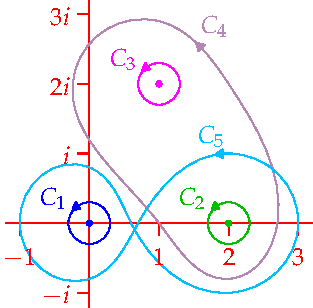
\includegraphics{res1}
	\end{minipage}\medbreak
	since the latter three integrands are analytic on/inside $C_1$. Similarly,
	\[
		\oint_{C_2}f(z)\,\dz=5i\oint_{C_2}\frac{\dz}{z-2}=\textcolor{Green}{-10\pi},\qquad
		\oint_{C_3}f(z)\,\dz = \oint_{C_3}\frac{\dz}{z-1-2i}=\textcolor{Magenta}{2\pi i}
	\]
	The curves $C_4$ and $C_5$ are more interesting. Since $f(z)$ is analytic on and between $C_4$ and $C_2/C_3$, Cauchy--Goursat tells us that
	\[
		\oint_{C_4}f(z)\,\dz
		=\oint_{C_2}f(z)\,\dz+\oint_{C_3}f(z)\,\dz
		=\textcolor{Green}{-10\pi}+\textcolor{Magenta}{2\pi i}
		=2\pi(i-5)
	\]
	$C_5$ appears trickier, though it becomes easy once you visualize it as \emph{two} contours: the first encircles \textcolor{Green}{$z_2=2$} \emph{counter-clockwise} while the second passes \emph{clockwise} around \textcolor{blue}{$z_1=0$}. We conclude that
	\[
		\int_{C_5}f(z)\,\dz
		=\oint_{C_2}f(z)\,\dz-\oint_{C_1}f(z)\,\dz
		=\textcolor{Green}{-10\pi}-\textcolor{blue}{6\pi i}
		=-2\pi(5+3i)
	\]
\end{example}

The example suggests that the value of any integral round a simple closed contour can be evaluated as a linear combination
\[
	\int_C f(z)\,\dz
	=\lambda_1\textcolor{blue}{\oint_{C_1}f}
	+\lambda_2\textcolor{Green}{\oint_{C_2}f}
	+\lambda_3\textcolor{Magenta}{\oint_{C_3}f}
	=\textcolor{blue}{6\pi i}\lambda_1
	\,\textcolor{Green}{-10\pi}\lambda_2
	+\textcolor{Magenta}{2\pi i}\lambda_3
\]
where $\lambda_k$ denotes the number of times $C$ orbits $z_k$ in a counter-clockwise direction.\goodbreak

%\boldsubsubsection{Isolated Singularities and their Types}

To properly develop the idea in the example, some new language is helpful.

\begin{defn}{Isolated Singularities}{isolated}
	We say that $z_0$ is an \emph{isolated singularity} of $f(z)$ if the function is analytic on a punctured disk $0<\nm{z-z_0}<R$, but not at $z_0$ itself.\par
	\begin{minipage}[t]{0.75\linewidth}\vspace{-2pt}
		By Laurent's Theorem (\ref{thm:laurent}), $f(z)$ equals its Laurent series on this domain:
		\[
			f(z)=\sum_{n=-\infty}^\infty a_n(z-z_0)^n
			\quad \text{where}\quad 
			a_n=\frac 1{2\pi i}\oint_C\frac{f(z)}{(z-z_0)^{n+1}}\,\dz
		\]
		and $C$ encircles $z_0$. The \emph{residue} of $f(z)$ at $z_0$ is the $-1$-coefficient
		\[
			\Resl{z=z_0}f(z)=a_{-1}=\frac 1{2\pi i}\oint_C f(z)\,\dz
		\]
	\end{minipage}
	\hfill
	\begin{minipage}[t]{0.24\linewidth}\vspace{-15pt}
		\flushright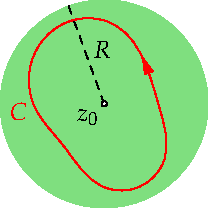
\includegraphics[scale=0.95]{isolatedsing}
	\end{minipage}\bigbreak
	The type of isolated singularity is determined by the rest of the Laurent series:
	\begin{description}
		\item[\normalfont\emph{Removable Singularity}] The Laurent series is a Taylor series (the residue is necessarily zero). There are no negative powers; the series $f(z)$ extends analytically to $z_0$. 
		\item[\normalfont{\emph{Pole of order $m$}}] The highest negative power in the Laurent series is $(z-z_0)^{-m}$. A pole of order 1 is typically called a \emph{simple pole,} order 2 a \emph{double pole,} etc.
		\item[\normalfont\emph{Essential Singularity}] The Laurent series has infinitely many negative terms.
	\end{description}
	% We may also consider the point at $\infty$ to be an isolated singularity, provided $f(z)$ is analytic for all large $z$: i.e.\ when $\nm z>R$.
\end{defn}


\begin{examples}{}{res2}
	\exstart The series $f(z)=\sum\limits_{n=0}^\infty 3^{-n}(z-2i)^n$ defined on the punctured disk $0<\nm{z-2i}<3$ has a removable singularity at $z_0=2i$ (residue $\smash{\Res\limits_{z=2i}f(z)=0}$). Indeed the function is a geometric series and thus equals
  \[
  	f(z)=\frac 1{1-\frac{z-2i}3}=\frac 3{3+2i-z}
  \]
  on the punctured disk. Certainly this extends analytically to $f(2i)=1$.
	\begin{enumerate}\setcounter{enumi}{1}
	  \item $\displaystyle e^{1/z}=\sum\limits_{n=0}^\infty\frac{z^{-n}}{n!}=1+\frac{\textcolor{red}{1}}z+\frac 1{2z^2}+\cdots$ has an essential singularity at zero with $\Res\limits_{z=0}e^{1/z}=\textcolor{red}{1}$.
	  
	  \item (Example \ref{ex:res1})\lstsp The function $f(z)=\frac 3{z}+\frac 1{z^2}+\frac{5i}{z-2}+\frac 1{z-1-2i}$ is analytic on the punctured disk $0<\nm{z}<0.3$ (inside the circle \textcolor{blue}{$C_1$}). Since $\frac{5i}{z-2}+\frac 1{z-1-2i}$ is also analytic at zero, the Laurent series of $f(z)$ about \textcolor{blue}{$z_1=0$} has the form
	  \[
	  	f(z)=\frac 1{z^2}+\frac 3{z}+\sum_{n=0}^\infty a_nz^n
	  \]
	  We conclude that $f(z)$ has a pole of order 2 at \textcolor{blue}{$z_1=0$} and residue $\smash{\Res\limits_{z=0}f(z)=\textcolor{blue}{3}}$. Similarly, $f(z)$ has simple poles (order 1) at \textcolor{Green}{$z_2=2$} and \textcolor{Magenta}{$z_2=1+2i$} with
	  \[
	  	\Resl{z=2}f(z)=\textcolor{Green}{5i},\qquad\Resl{z=1+2i}f(z)=\textcolor{Magenta}{1}
	  \]
	\end{enumerate}
\end{examples}


%In our motivating example (\ref{ex:res1}), we essentially saw that residues can be summed. More generally we have the following key result. 

\begin{thm}[lower separated=false, sidebyside, sidebyside align=top seam, sidebyside gap=0pt, righthand width=0.3\linewidth]{Cauchy's Residue Theorem}{}
	Let $f(z)$ be analytic on and inside a simple closed contour $C$, except at finitely many singularities $z_1,\ldots,z_n$. Then
	\[
		\oint_Cf(z)\,\dz=2\pi i\sum_{k=1}^n\Resl{z=z_k}f(z)
	\]
	More generally, if $C$ is closed and orbits the point $z_k$ counter-clockwise $\lambda_k$ times (the \emph{winding number} of $C$ about $z_k$), then
	\[
		\int_Cf(z)\,\dz=2\pi i\sum_{k=1}^n\lambda_k\Resl{z=z_k}f(z)
	\]
	\tcblower
	\flushright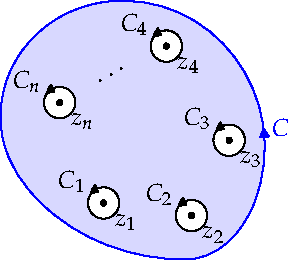
\includegraphics[scale=0.95]{res2}
\end{thm}


\begin{proof}
	First, center a circle $C_k$ at each $z_k$ such that no other singularities lie on/inside $C_k$ and apply Cauchy--Goursat. The general argument follows by considering paths like $C_5$ in Example \ref{ex:res1}. 
\end{proof}


\begin{examples}{}{res3}
	Let $C$ be the circle with radius 4 centered at the origin and $E$ the green curve drawn.
	\begin{enumerate}
	  \item The rational function $\smash{f(z)=\frac{3(1+iz)}{z(z-3i)}}$ has simple poles at $z_1=0$ and $z_2=3i$. There are several ways to compute the residues and thus the integrals $\oint_Cf(z)\dz$ and $\oint_Ef(z)\dz$.\smallbreak
		\begin{minipage}[t]{0.67\linewidth}\vspace{-10pt}
			\emph{Partial Fractions}\quad It's just high-school algebra!
			\begin{align*}
				f(z)=\frac iz+\frac{2i}{z-3i} &\implies \Resl{z=0} f(z)=i,\quad \Resl{z=3i} f(z)=2i\\
				&\implies \oint_Cf(z)\,\dz=2\pi i(i+2i)=-6\pi
			\end{align*}
			The curve $E$ orbits \emph{twice clockwise} around $z_1$ and \emph{once counter-clockwise} around $z_2$. Thus
			\[
				\int_Ef(z)\,\dz=2\pi i\left[-2\Resl{z=0} f(z)+\Resl{z=3i}f(z)\right] =0
			\]
		\end{minipage}
		\hfill
		\begin{minipage}[t]{0.32\linewidth}\vspace{0pt}
			\flushright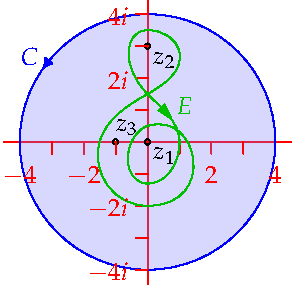
\includegraphics[scale=0.95]{res3}
		\end{minipage}\medbreak
	
		\emph{Laurent series}\quad Remember that we only need to find the $z^{-1}$ terms for the \textcolor{red}{residues}!
		\begin{gather*}
		  \frac{3(1+iz)}{z(z-3i)}
		  	=\frac{i-z}{z(1-\frac{iz}3)}
		  	=\left(\frac iz-1\right)\sum_{n=0}^\infty\left(\frac{iz}3\right)^n 
		  	=\frac{\textcolor{red}{i}}z+\text{power series}\\
		  \frac{3(1+iz)}{z(z-3i)}
		  	=\frac{z-3i+2i}{(1+\frac{z-3i}{3i})(z-3i)}
		  	=\left(\frac{2i}{z-3i}+1\right)\sum_{n=0}^\infty\left(\frac{3i-z}{3i}\right)^n 
		  	=\frac{\textcolor{red}{2i}}{z-3i}+\text{power series}
		\end{gather*}
	  
		\emph{Cauchy's integral formula}\quad Let $C_k$ be a small circle around $z_k$, then
		\begin{gather*}
		  \Res_{z=0}f(z)=\frac 1{2\pi i}\oint_{C_1}f(z)\,\dz 
		  	=\frac 1{2\pi i}\oint_{C_1}\frac{3(1+iz)}{z(z-3i)}\,\dz 
		  	=\frac{3(1+iz)}{z-3i}\bigg|_{z=0}=i\\
		  \Res_{z=3i}f(z)=\frac 1{2\pi i}\oint_{C_2}f(z)\,\dz 
		  =\frac 1{2\pi i}\oint_{C_2}\frac{3(1+iz)}{z(z-3i)}\,\dz 
		  =\frac{3(1+iz)}{z}\bigg|_{z=3i}=2i
		\end{gather*}
		%We'll revisit this last approach in the next section.
	  \goodbreak
	  
	  \item $f(z)=z^2\sin\frac 1z$ has one isolated singularity at the origin. Using the Maclaurin series for $\sin z$, we see that this is an essential singularity. Moreover,
	  \[
	  	z^2\sin\frac 1z=\sum_{n=0}^\infty \frac{(-1)^n}{(2n+1)!}z^{1-2n} \implies \oint_Cz^2\sin\frac 1z\,\dz=2\pi i\Resl{z=0}\left(z^2\sin\frac 1z\right) =-\frac{\pi i}3
	  \]
	  Since $E$ loops \textcolor{red}{twice clockwise} around the origin, we obtain
	  \[
	  	\int_Ez^2\sin\frac 1z\,\dz=2\pi i\cdot (\textcolor{red}{-2})\Resl{z=0}\left(z^2\sin\frac 1z\right) =\frac{2\pi i}3
	  \]  
	
		\item $f(z)=3e^{1/z}+\frac 4{z-7i}+\frac{2i}{z+1}$ has an essential singularity at the origin and two simple poles at $-1$ and $7i$. Since the last of these lies \emph{outside} the curves $C,E$, it does not contribute to either integral. Moreover, since $E$ loops \textcolor{red}{twice clockwise} around the origin and \textcolor{blue}{once clockwise} around $z_3=-1$. We therefore have
	  \begin{gather*}
	  	\oint_Cf(z)\,\dz
	  		=2\pi i\left(\Resl{z=0}3e^{1/z}+\Resl{z=-1}\frac{2i}{z+1}\right)
	  	=	2\pi i(3+2i)\\
	  	\oint_Ef(z)\,\dz
	  		=2\pi i\left(\textcolor{red}{-2}\Resl{z=0}3e^{1/z} +(\textcolor{blue}{-1})\Resl{z=-1}\frac{2i}{z+1}\right)
	  		=2\pi i(-6-2i)=4\pi(1-3i)
	  \end{gather*}
	\end{enumerate}
\end{examples}

\goodbreak

\boldsubsubsection{Non-isolated Singularities}

Revisit Definition \ref{defn:isolated}. A point $z_0$ is said to be a \emph{non-isolated singularity} of $f(z)$ if the function is non-analytic (including undefined) at $z_0$ and at some point on \emph{every} punctured disk $0<\nm{z-z_0}<R$. Such a function is necessarily non-analytic at infinitely many points and does not have a Laurent series centered at $z_0$. Non-isolated singularities typically appear in two flavors.

\begin{examples}{}{}
	\exstart $f(z)=\bigl(\polar{2\pi i}z-1\bigr)^{-1}$ has singularities at \textcolor{Green}{$z_0=0$} and at \textcolor{blue}{$z_n=\frac 1n$} for each non-zero integer $n$. Each \textcolor{blue}{non-zero singularity} is isolated (choose e.g., \textcolor{blue}{$R_n=\frac 1{(\nm n+1)^2}$} in Definition \ref{defn:isolated}). The \textcolor{Green}{\emph{limit point} $z_0=0$} is non-isolated: for any $R>0$, the \textcolor{Green}{punctured disk} $0<\nm z<R$ contains \textcolor{blue}{other singularities}.
	\begin{center}
		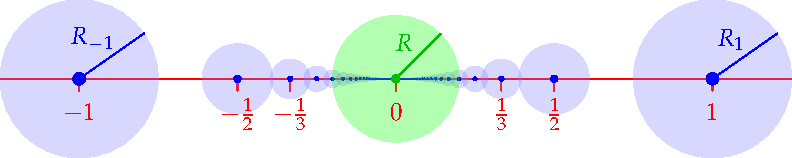
\includegraphics[scale=0.95]{sing1}
	\end{center}
	
	\begin{enumerate}\setcounter{enumi}{1}
		\begin{minipage}[t]{0.72\linewidth}\vspace{0pt}
		  \item The square-root function $f(z)=z^{1/2}$ has a \textcolor{Green}{\emph{branch point}} $z_0=0$. For $f$ to be analytic, we need to make a branch cut: for instance the \textcolor{blue}{non-positive real axis} for the principal branch.\par
		  Since any \textcolor{Green}{punctured disk} $0<\nm z<R$ contains other points of the \textcolor{blue}{branch cut} (where $f$ is non-analytic), the branch point is a non-isolated singularity \emph{for any branch} of $f$.\par
		\end{minipage}
		\hfill
		\begin{minipage}[t]{0.25\linewidth}\vspace{0pt}
			\flushright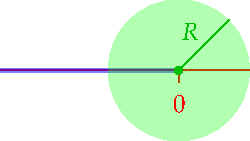
\includegraphics[scale=0.95]{sing2}
		\end{minipage}
	\end{enumerate}
\end{examples}


\goodbreak


\begin{exercises}
	\exstart For each type of singularity, what, if anything, can be said about the value of the residue $\Res\limits_{z=z_0}f(z)$? Choose from `Equals zero,' `Non-zero,' or `No restriction'.\vspace{-5pt}
	\begin{enumerate}\setcounter{enumi}{1}
	  \item[]\begin{enumerate}
		  \item \makebox[200pt][l]{Removable singularity. \hfill (b) }\ Simple pole.
		  \setcounter{enumii}{2}
		  \item \makebox[200pt][l]{Pole of order $m\ge 2$. \hfill (d) }\ Essential singularity.
		\end{enumerate}
		
	  \item	Find the residue at $z=0$ of each function:
	  \begin{enumerate}
	    \item $f(z)=\dfrac 1{z+3z^2}$\qquad 
	    (b)\ \ $\displaystyle g(z)=z\cos\frac 1z$\qquad 
	    (c) \ \ $h(z)=\dfrac{z-\sin z}{z}$
		\end{enumerate}
		
		\item Let $C$ be the circle $\nm z=3$. Evaluate the integrals using Cauchy's residue theorem:
	  \begin{enumerate}
	    \item $\displaystyle\oint_C\frac{e^{-z}}{z^2}\,\dz$\qquad 
	    (b)\ \ $\displaystyle\oint_C\frac{e^{-z}}{(z-1)^2}\,\dz$\qquad 
	    (c) \ \ $\displaystyle\oint_Cz^2e^{1/z}\,\dz$\qquad 
	    (d)\ \ $\displaystyle\oint_C\frac{z+1}{z^2-2z}\,\dz$
		\end{enumerate}
		
		
		\item Suppose a closed contour $C$ loops twice counter-clockwise around $z=i$ and three times clockwise around $z=2$. Use residues to compute the integral
		\[
			\int_C\frac{z+3}{(z-2)^2(z-i)}\,\dz
		\]
		
		
		\item Identify the type of singular point of each function and determine the residue:
		\begin{enumerate}
		  \item $\dfrac{1-\cosh z}{z^3}$\qquad 
		  (b)\ \ $\dfrac{1-e^{2z}}{z^4}$\qquad 
		  (c)\ \ $\dfrac{e^{2z}}{(z-1)^2}$
		\end{enumerate}
		
		
		\item\label{exs:analytictopole} Suppose $f(z)$ is analytic at $z_0$ and define $g(z)=(z-z_0)^{-1}f(z)$. Prove:
		\begin{enumerate}
		  \item If $f(z_0)\neq 0$, then $z_0$ is a simple pole of $g(z)$ with $\Res\limits_{z=z_0}g(z)=f(z_0)$;
		  
		  \item If $f(z_0)= 0$, then $z_0$ is a removable singularity of $g(z)$.
		\end{enumerate}
		
		
		\item\label{exs:resinfinity} A function $f(z)$ is said to have an \emph{isolated singularity at $\infty$} if it is analytic on some infinite annulus $\nm{z}>R$. On this domain, we have a Laurent series $f(z)=\sum_{n=-\infty}^\infty a_nz^n$.
		\begin{enumerate}
		  \item What properties do you think this series should have if we were to describe the singularity at $\infty$ to be:
		  \begin{enumerate}
		    \item Removable?\qquad ii.\ \ A pole of order $m$?\qquad iii.\ \ Essential?
		  \end{enumerate}
	
		  \item The \emph{residue at $\infty$} of the above function is defined to be
		\[
			\Res_{z=\infty}f(z):=-\Res_{z=0}\left(z^{-2}f(z^{-1})\right) \tag{$\ast$}
		\]
		 	\begin{enumerate}
		    \item Prove that $\Res\limits_{z=\infty}f(z)=-a_{-1}$, where $a_{-1}$ is the coefficient in the above Laurent series.%$For example $\Resl{z=\infty}\frac{z^2+1}{z^3}=-1$.
	
		    \item Suppose $f(z)$ is analytic on $\C$ except at finitely many singularities. By substituting $w=\frac 1z$ in ($\ast$), prove that the \emph{sum} of all residues, \emph{including at infinity}, is zero.
		  \end{enumerate}
		\end{enumerate}
	
		
		\item Let $P(z)$ and $Q(z)$ be polynomials and assume $C$ is a simple closed contour such that all zeros of $Q(z)$ lie interior to $C$.
		\begin{enumerate}
		  \item If $\deg Q\ge 2+\deg P$, prove that $\oint_C\frac{P(z)}{Q(z)}\,\dz=0$
			
			\item What can you conclude if $\deg Q=1+\deg P$?
		\end{enumerate}
		(\emph{Hint: Combine Exercises \ref*{exs:analytictopole} \& \ref*{exs:resinfinity}, or try the substitution $w=\frac 1z$ directly})

	\end{enumerate}
\end{exercises}


\clearpage




\subsection{Poles \& Zeros}


If the order of a pole is known, residues may often be computed quite efficiently. For instance, if $f(z)$ has a pole of order $m$, Laurent's Theorem tells us that
\[
	f(z)=\sum_{n=-m}^\infty a_n(z-z_0)^n =(z-z_0)^{-m}\phi(z),
	\quad\text{where}\quad
	\phi(z)=\sum_{n=0}^\infty a_{n-m}(z-z_0)^n \tag{$\ast$}
\]
Plainly $\phi(z)$ is analytic at $z_0$ and $\phi(z_0)=a_{-m}\neq 0$. In fact this property categorizes poles of order $m$ (analogous to Theorem \ref{thm:zerocategorize} for zeros), providing a simple formula for the computation of residues. 


\begin{thm}{}{polesimple}
	A function $f(z)$ has a pole of order $m$ at $z_0$ if and only if $f(z)=(z-z_0)^{-m}\phi(z)$ where $\phi(z)$ is \emph{analytic} at $z_0$ and $\phi(z_0)\neq 0$. In such situations, the residue is a Taylor coefficient of $\phi(z)$:\footnotemark
	\[
		f(z)=(z-z_0)^{-m}\sum_{n=0}^\infty \frac{\phi^{(n)}(z_0)}{n!}(z-z_0)^n \implies \Res_{z=z_0}f(z)=\frac 1{(m-1)!}\phi^{(m-1)}(z_0)
	\]
	This specializes to $\Res\limits_{z=z_0}f(z)=\phi(z_0)$ for a simple pole.
\end{thm}


\footnotetext{\label{fn:bob}The formula works whenever $f(z)=(z-z_0)^{-m}\phi(z)$ with $\phi$ analytic, \textbf{even if $\boldsymbol{\phi(z_0)=0}$}. However, a naïve application means you won't know the order of the pole and you'll have to differentiate more times than necessary!}

\begin{proof}
	The $(\Rightarrow)$ direction is above. For the converse: $\phi(z)$ equals its Taylor series and so ($\ast$) describes the Laurent series of $f(z)=(z-z_0)^{-m}\phi(z)$ (Corollary \ref{cor:laurenttidy}, uniqueness), which moreover has a pole of order $m$ since $a_{-m}=\phi(z_0)\neq 0$.
\end{proof}

\begin{examples}{}{polecalceasy}
	\exstart (Example \ref{ex:res3} revisited)\lstsp $f(z)=\smash{\frac{3(1+iz)}{z(z-3i)}}$ has two poles:
	\begin{enumerate}\setcounter{enumi}{1}
		\item[]\begin{description}
			\item[\normalfont\emph{Simple pole at $z_1=0$}:] Write $f(z)=z^{-1}\phi_1(z)$, where $\phi_1(z)=\frac{3(1+iz)}{z-3i}$. This is analytic and non-zero at $z_1=0$, whence
\[\Res\limits_{z=0}f(z)=\phi_1(0)=\frac 3{-3i}=i\]
			\item[\normalfont\emph{Simple pole at $z_2=3i$}:] This time, $f(z)=(z-3i)^{-1}\phi_2(z)$, where $\phi_2(z)=\frac{3(1+iz)}{z}$. Thus
			\[
				\Res\limits_{z=3i}f(z)=\phi_2(3i)=\frac{3(1-3)}{3i}=2i
			\]
	  \end{description}
	  
	  \item $f(z)=\frac{1-2iz}{(z-1)(z-2i)^3}$ also has two poles.
	  \begin{description}
			\item[\normalfont\emph{Simple pole at $z_1=1$}:] Write $f(z)=(z-1)^{-1}\phi_1(z)$, where $\phi_1(z)=\frac{1-2iz}{(z-2i)^3}$. Thus 
	    \[
	    	\Resl{z=1}f(z) =\phi_1(1)
	    	=\frac{1-2i}{(1-2i)^3} =\frac 1{(1-2i)^2}
	    	=\frac{4i-3}{25}
	    \]
			\item[\normalfont\emph{Pole of order three at $z_2=2i$}:] $f(z)=(z-2i)^{-1}\phi_2(z)$, where $\phi_2(z)=\frac{1-2iz}{z-1}=-2i+\frac{1-2i}{z-1}$. Thus
		  \[
		    \Resl{z=2i}f(z) =\frac 1{(3-1)!}\phi_2''(2i)
		    =\frac{1-2i}{(z-1)^3}\bigg|_{z=2i}
		    =\frac{-1}{(2i-1)^2} =\frac{3-4i}{25}
		  \]
	  \end{description}
	\end{enumerate}
\end{examples}

\goodbreak

As the previous examples show, the method is very effective for rational with low-order poles; as a bonus, it saves us from partial fractions! Its utility is more variable for other functions\ldots

\begin{examples}{}{residuesdiffmethod}
	\exstart The function $f(z)=\frac{e^z}{(z-1)^2(z+1)}=(z-1)^{-2}\phi(z)$
	has a double pole at $z_0=1$, with
	\[
		\Resl{z=1}f(z)=\frac 1{(2-1)!}\phi'(1)=\frac{ze^z}{(z+1)^2}\bigg|_{z=1} =\frac 14e
	\]
	\begin{enumerate}\setcounter{enumi}{1}
	  \item\label{ex:residuesdiffmethod2} Don't let the denominator fool you! At first glance we appear to have a pole of order \emph{six}: 
		\[
			f(z)=\frac{6\sin z-6z+z^3}{z^6}=\frac{\smash[t]{\widetilde\phi(z)}}{z^6}\overset{\text{??}}{\implies} \Resl{z=0}f(z)=\frac 1{5!}\widetilde\phi^{(5)}(0)=\frac 6{120}=\frac 1{20}
		\]
		However, if we apply the Maclaurin series for sine, we instead find a \emph{simple pole}:
		\begin{align*}
		  f(z)&=\frac 1{z^6}\left(6\sum_{n=0}^\infty\frac{(-1)^n}{(2n+1)!}z^{2n+1}-6z+z^3\right)
		  =z^{-6}\sum_{n=2}^\infty\frac{6(-1)^n}{(2n+1)!}z^{2n+1}\\
		  &=z^{-1}\textcolor{blue}{\sum_{m=0}^\infty\frac{6(-1)^m}{(2m+5)!}z^{2m}}
		  =\frac 1{20z}+\frac 1{840}+\cdots
		  \implies \Resl{z=0}f(z)=\frac 1{20}
	  \end{align*}
	  Even though the first calculation produced the correct residue (see footnote \ref{fn:bob}), the function $\smash[t]{\widetilde\phi}$ was incorrect ($\smash[t]{\widetilde\phi}(0)=0$). The correct function is the series \textcolor{blue}{$\phi(z)=6\sum\limits_{m=0}^\infty\frac{(-1)^m}{(2m+5)!}z^{2m}$}.
	\end{enumerate}
\end{examples}





% \boldsubsubsection{Relating and Counting Poles and Zeros}

% It seems intuitive that we can turn poles into zeros just by flipping a function upside down.
% 
% \begin{lemm}{}{polezeroreverse}
% 	Let $f(z)$ be analytic at $z_0$ and define $g(z)=\frac 1{f(z)}$. Then, at $z_0$,
% 	\[
% 		f(z)\text{ has a zero of order }m\iff g(z)\text{ has a pole of order }m
% 	\] 
% \end{lemm}

% \begin{proof}
% Write $f(z)=(z-z_0)^m\psi(z)$ and $g(z)=(z-z_0)^{-m}\phi(z)$ where $\phi(z)=\frac 1{\psi(z)}$. Then\vspace{-2pt}
% \[\psi(z)\text{ is analytic and non-zero at }z_0\iff \phi(z)\text{ is also}\tag*{\qedhere}\]
% \end{proof}

%The proof is a simple exercise combining Theorems \ref{thm:zerocategorize} \& \ref{thm:polesimple}. 

For certain functions with \emph{simple poles}, the method is even easier.

\begin{cor}{}{easyres}
	Suppose $p(z)$, $q(z)$ are analytic at $z_0$, that $p(z_0)\neq 0$ and that $q(z)$ has a simple zero. Then $f(z)=\frac{p(z)}{q(z)}$ has a simple pole at $z_0$, and
	\[
		\Resl{z=z_0}\frac{p(z)}{q(z)} =\frac{p(z_0)}{q'(z_0)}
	\]
\end{cor}

\begin{proof}
	By Theorem \ref{thm:zerocategorize}, $q(z)=(z-z_0)\psi(z)$ where $\psi$ is analytic and $\psi(z_0)\neq 0$. Take $\phi(z)=\frac{p(z)}{\psi(z)}$ in Theorem \ref{thm:polesimple} ($\phi$ is analytic and non-zero at $z_0$), to see that
	\[
		f(z)=\frac{p(z)}{q(z)}=(z-z_0)^{-1}\frac{p(z)}{\psi(z)}
		\qquad \text{and}\qquad
		\Resl{z=z_0}\frac{p(z)}{q(z)}=\phi(z_0)
		=\frac{p(z_0)}{\psi(z_0)}=\frac{p(z_0)}{q'(z_0)}
		\tag*{\qedhere}
	\]
\end{proof}


\begin{examples}{}{}
% 	\exstart The function $f(z)=\frac{p(z)}{q(z)}=\frac{(z^2+1)^2}{z-3}=\frac{(z-i)^2(z+i)^2}{z-3}$ has zeros of order two at $\pm i$ and a simple pole at $z=3$. The reciprocal has the reverse arrangement: poles of order two at $\pm i$ and a simple zero at $3$. Moreover,
%   \[\Resl{z=3}f(z)=\frac{p(3)}{q'(3)}=\frac{(3^2+1)^2}{1}=100\]
	\exstart The function $f(z)=\frac{p(z)}{q(z)}=\frac{\sin z}{z^2+4} =\frac{\sin z}{(z-2i)(z+2i)}$ has simple poles at $\pm 2i$ with 
  \[
  	\Resl{z=2i}f(z)=\Resl{z=-2i}f(z)
  	=\frac{p(\pm 2i)}{q'(\pm 2i)}
  	=\frac{\sin 2i}{4i}=\frac 18(e^2-e^{-2}) =\frac 14\sinh 2
  \]
  The reciprocal $g(z)=\frac{q(z)}{p(z)} =\frac{z^2+4}{\sin z}$ has simple poles at $z=n\pi$ for every $n\in\Z$, with
  \[
  	\Resl{z=n\pi}\frac{z^2+4}{\sin z}
  	=\frac{q(n\pi)}{p'(n\pi)}
  	=\frac{n^2\pi^2+4}{\cos n\pi}
  	=(-1)^n(n^2\pi^2+4)
  \]
	\begin{enumerate}\setcounter{enumi}{1}
	  \item Since $q(z)=e^{2z}-1=\sum\limits_{n=1}^\infty\frac{2^nz^n}{n!}=z\sum\limits_{n=0}^\infty\frac{2^nz^n}{(n+1)!}$ has a simple zero at $z=0$, we see that
	  \[
	  	f(z)=\frac{\sqrt{z+4i}}{(z+i)^2\Log(z+2)(e^{2z}-1)}=\frac{p(z)}{q(z)} 
	  	\tag*{$\left(p(z)=\frac{\sqrt{z+4i}}{(z+i)^2\Log(z+2)}\right)$}
	  \]
	  has a simple pole at $z=0$ and may easily compute
	  \[
	  	\Resl{z=0}f(z)=\frac{p(0)}{q'(0)}=\frac{\polar{i\pi}4}{\ln 2} =\frac{1+i}{\sqrt 2\ln 2}
	  \]
	  We could instead have chosen $q(z)=(z+i)^2\Log(z+2)(e^{2z}-1)$, but computing $q'(z)$ would have been disgusting!
	\end{enumerate}
\end{examples}


\boldsubsubsection{Counting the Number of Poles and Zeros}

A sneaky application of our pole/zero categorization permits us to \emph{count} them.\smallbreak

Suppose $f$ has a zero of order $m$ at $z_0$. Write $f(z)=(z-z_0)^m\psi(z)$ where $\psi(z)$ is analytic and \emph{non-zero} on some closed disk $\nm{z-z_0}\le R$. Let $C_0$ be the boundary of the disk and compute:
	\begin{align*}
		\oint_{C_0}\frac{f'(z)}{f(z)}\,\dz
		&=\oint_{C_0}\frac{m(z-z_0)^{m-1}\psi(z)+(z-z_0)^m\psi'(z)}{(z-z_0)^m\psi(z)} \,\dz\\
		&=\oint_{C_0}\frac m{z-z_0}+\frac{\psi'(z)}{\psi(z)}\,\dz
		=2\pi im
	\end{align*}
	where we used the fact that $\frac{\psi'(z)}{\psi(z)}$ is analytic on and inside $C_0$.	The integral $\frac 1{2\pi i}\oint_{C_0}\frac{f'(z)}{f(z)}\,\dz$ therefore counts the \emph{multiplicity} of the zero. By performing a similar calculation for poles and combining the results for several poles and zeros, we recover a famous result.

	
\begin{thm}{Cauchy's Argument Principle}{argprinciple}
	Suppose $f$ is analytic except at poles,\footnotemark{} on and inside a simple closed curve $C$, and that $f(z)$ has no poles or zeros on $C$. Then
	\[
		\frac 1{2\pi i}\oint_C\frac{f'(z)}{f(z)}\,\dz =Z-P
	\]
	where $Z$ and $P$ are the number of zeros and poles of $f$ inside $C$, counted up to multiplicity.
\end{thm}

\footnotetext{Such a function is termed \emph{meromorphic.} The result is called the argument principle because $\frac{f'(z)}{f(z)}=\diff z\log f(z)$ means that the integral is calculating the net change in the logarithm, and thus \emph{argument}, of $f(z)$ round the curve $C$. }


\begin{example}{}{}
	Consider $f(z)=\frac{(z-i)^2\sin z}{(z-5)^4}$ where $C$ is a large circle surrounding the points 0, $i$ and 5. Plainly $Z=2+1=3$ and $P=4$. We may compute the integral explicitly,
	\[
		\frac 1{2\pi i}\oint_C\frac{f'(z)}{f(z)}\,\dz =\frac 1{2\pi i}\oint_C\frac 2{z-i}+\frac{\cos z}{\sin z}-\frac 4{z-5}\,\dz =2+\cos 0-4=-1 =Z-P
	\]
	(Use logarithmic differentiation unless you're feeling masochistic!)
\end{example}

\goodbreak


\boldsubsubsection{Properties of Isolated Singularities}

Recall (Definition \ref{defn:isolated}) that a function $f(z)$ analytic on a punctured disk $0<\nm{z-z_0}<R$ can have one of three types of isolated singularity at $z_0$: removable, pole, and essential. We finish by considering some conditions/properties for each type.

\begin{thm}{Removable Singularities}{}
	Suppose $f(z)$ has an isolated singularity at $z_0$. The following are equivalent:
	\begin{enumerate}
		\item The singularity is removable.
		\item \smash[b]{$\lim\limits_{z\to z_0}f(z)$} exists and is finite.
		\item There exists a punctured disk $0<\nm{z-z_0}<\delta$ on which $f(z)$ is bounded.
	\end{enumerate}
\end{thm}

\begin{proof}
	For simplicity, suppose that $z_0=0$ and that $f(z)$ is analytic on the punctured disk $0<\nm z<R$.
	\begin{description}
	  \item[$(1\Rightarrow 2)$] Since $z_0$ is removable, the Laurent series \smash[b]{$f(z)=\sum\limits_{n=0}^\infty a_nz^n$} on $0<\nm z<R$ has no negative terms. It follows that \smash[b]{$\lim\limits_{z\to 0}f(z)=a_0$}.
		\item[$(2\Rightarrow 3)$] This is almost tautological but bears repeating: If \smash[b]{$\lim\limits_{z\to 0}f(z)=a_0$} is finite then choose $\epsilon=\nm{a_0}$ in the definition;
		\begin{align*}
			\exists \delta>0\text{ such that }0<\nm z<\delta&\implies \nm{f(z)-a_0}<\nm{a_0}\\
			&\implies \nm{f(z)}=\nm{f(z)-a_0+a_0}\overset{\triangle}{<}2\nm{a_0}
		\end{align*}
		\item[$(3\Rightarrow 1)$] Suppose $f(z)$ is bounded on $0<\nm z<\delta$, and consider
		\[
			g(z)=
			\begin{cases}
				z^2f(z)&\text{if }0<z<\delta\\
				0&\text{if }z=0
			\end{cases}
		\]
		Since $f$ is bounded, we may compute the limit
		\[
			\lim_{z\to 0}\frac{g(z)-g(0)}{z}=\lim_{z\to 0}zf(z)=0
		\]
		whence $g(z)$ is differentiable at zero! Since $g(z)$ is already differentiable on the punctured disk $0<\nm z<\min(\delta,R)$, it is therefore analytic on the \emph{disk} $\nm z<\min\{\delta,R\}$ and equals its Maclaurin series
		\[
			g(z)=\sum_{n=0}^\infty b_nz^n
			=\sum_{n=2}^\infty b_nz^n =z^2\sum_{m=0}^\infty b_{m-2}z^m
			\tag{$b_0=g(0)=0$ and $b_1=g'(0)=0$}
		\]
		We conclude that
		\[
			f(z)=\sum_{m=0}^\infty b_{m-2}z^m
			\quad\text{whenever}\quad
			0<\nm z<\min(\delta,R)
		\]
		whence $f$ has a removable singularity at zero.\qedhere
	\end{description}
\end{proof}

\goodbreak

We leave the next result as an exercise.

\begin{thm}{}{casorati}
	Suppose $f$ has an isolated singularity at $z=z_0$.
	\begin{enumerate}
	  \item $z_0$ is a pole if and only if \smash[b]{$\lim\limits_{z\to z_0}f(z)=\infty$.}
	  \item Suppose $z_0$ is essential and that $w\in\C\cup\{\infty\}$ is given. Then there exists a sequence $(z_n)$ converging to $z_0$ for which $\lim\limits_{n\to\infty} f(z_n)=w$. 
	\end{enumerate}
\end{thm}

Combined with the previous result, we see that $z_0$ is an essential singularity if and only if \smash[b]{$\lim\limits_{z\to z_0}f(z)$} does not exist.\smallbreak

The second result is the \emph{Casorati--Weierstrass Theorem}; the range of $f(z)$ is \emph{dense} in any neighborhood of an essential singularity. A stronger result is available, through its proof is beyond us.

\begin{thm}{Picard}{}
	If $z_0$ is an essential singularity of $f(z)$, then, on any neighborhood of $z_0$, $f(z)$ takes every complex value \emph{except at most one}.
\end{thm}

\begin{example}{}{}
	We verify Picard's Theorem for the essential singularity of $f(z)=e^{1/z}$ at $z_0=0$. Let $w\in\C\setminus\{0\}$ be given, and write $w=re^{i\theta}$ where $0\le \theta<2\pi$. Then
	\[
		f(z)=w\iff e^{1/z}=e^{\ln r+i\theta} \iff \frac 1z=\ln r+i\theta+2\pi in
	\]
	for some integer $n$. If $n>0$, observe that
	\[
		\nm{\frac 1z}=\sqrt{(\ln r)^2+(\theta+2\pi n)^2}\ge 2\pi n \implies \nm z<\frac 1{2\pi n}
	\]
	whence $\nm z$ can be chosen arbitrarily small. A suitable value $z$ therefore exists in any punctured disk $0<\nm z<\delta$. The function $f(z)=e^{1/z}$ thus takes on every complex value except one (namely $w=0$).
\end{example}



\begin{exercises}
	\exstart Determine the order of each pole and its residue.
	\begin{enumerate}\setcounter{enumi}{1}
	  \item[]\begin{enumerate}
	    \item $f(z)=\dfrac{z+1}{z^2+9}$\qquad\qquad
	    (b)\ \ $f(z)=\left(\dfrac{z}{2z+1}\right)^3$
	  \end{enumerate}
	  
	  
	  \item Verify the value of each residue:
	  \begin{enumerate}\itemsep4pt
	    \item $\displaystyle\Res\limits_{z=-1}\frac{z^{1/4}}{z+1}=\frac{1+i}{\sqrt 2}$ when $\nm z>0$ and $\arg z\in(0,2\pi)$
	    \qquad\qquad
	    (b) \  $\displaystyle\Res\limits_{z=i}\frac{\Log z}{(z^2+1)^2}=\frac{\pi+2i}8$
	    \setcounter{enumii}{2}
	    
	    \item $\displaystyle\Res\limits_{z=z_n}\bigl(z\sec z\bigl)=(-1)^{n+1}z_n$, where $z_n=\frac\pi 2+n\pi$ and $n\in\Z$
	  \end{enumerate}
	  
	  
	  \item Find the value of the integral round each circle:
	  \[
	  	\oint_C\frac{3z^3+2}{(z-1)(z^2+9)}\,\dz
	  \]
	 	(a) \ $\nm{z-2}=2$\qquad\qquad (b) \ $\nm z=4$
	  
	  
	  \item Let $C$ be the circle $\nm z=2$. Evaluate $\oint_C\tan z\,\dz$.
	  
	  
	  \item Suppose functions $f,g$ satisfy $g(z)=\frac 1{f(z)}$. Prove:
		\[
			\text{At $z_0$,}\quad f(z)\text{ has a zero of order $m$}\iff g(z)\text{ has a pole of order $m$}
		\] 

	  
	  \item\begin{enumerate}
	    \item Evaluate $\Res\limits_{z=\frac 1n}\left(z\sin\frac\pi z\right)^{-1}$ for each $n\in\Z$.
	    \item Why doesn't $\Res\limits_{z=0}\left(z\sin\frac\pi z\right)^{-1}$ make sense?
	  \end{enumerate}
		
	  	  
	  \item Suppose that $C$ is the rectangle whose sides are the lines $x=\pm 2, y=0$ and $y=1$. Prove that
	  \[
	  	\oint_C\frac{\dz}{(z^2-1)^2+3}=\frac\pi{2\sqrt 2}
	  \]
	  (\emph{Hint: the integrand has four simple poles, only two of which lie inside $C$})
	  
	  		  
	  \item (Hard)\lstsp Suppose $f(z)$ and the contour $C$ satisfy the hypotheses of Cauchy's Argument Principle (Theorem \ref{thm:argprinciple}).
	  \begin{enumerate}
	    \item Explain why we can be sure that there are only \emph{finitely many} poles/zeros inside $C$ and that all zeros are isolated.
	    \item Complete the proof of the argument principle by performing a suitable integral on a small circle round each pole and applying Cauchy--Goursat and/or the Residue Theorem. 
	    \item (Winding number)\lstsp Consider the curve $\gamma=f(C)$. By substituting $w=f(z)$, explain why $\frac 1{2\pi i}\oint_C\frac{f'(z)}{f(z)}\,\dz$ counts the number times $\gamma$ orbits the origin counter-clockwise.
	    \item\begin{enumerate}
	      \item (Rouché's Theorem)\lstsp Suppose $f$ is analytic on/inside $C$ and that $\nm{g(z)}<\nm{f(z)}$ for all $z\in C$. Prove that the number of zeros of $f+g$ inside $C$ equals that of $f$.\par
	    	(\emph{Hints: Apply the argument principle to $f+g=f\cdot(1+\frac gf)$ and consider why $1+\frac gf$ has winding number zero---why is $\Re(1+\frac gf)> 0$?})
	    	\item %Since $\nm{4z^3}>\nm{z^{22}+2i}$ on the circle $\nm z=1$, 
	    	How many solutions (up to multiplicity) are there to the equation $z^{22}+4z^3+2i=0$ on the domain $\nm z<1$?
	    \end{enumerate}
	  \end{enumerate}
	
	
		\item (Hard)\lstsp Prove both parts of Theorem \ref{thm:casorati}; for simplicity, assume $z_0=0$.
		\begin{description}  	
	  	\item[](\emph{Hint 1: $f(z)$ has a pole if and only if $\frac 1{f(z)}$ has a zero.}
	  	\item[]\,\emph{Hint 2: If no such sequence exists, show that $g(z):=\frac 1{f(z)-w}$ is analytic and bounded.})
		\end{description}
		
	\end{enumerate}
\end{exercises}


\clearpage



\subsection{Improper Integrals}

The theory of residues may be applied to help evaluate certain \emph{real} improper integrals. We start with an alternative definition of improper integral suited to our purposes.

\begin{defn}{}{}
	Suppose $f:\R\to\R$ is integrable. Provided the limit exists, the \emph{Cauchy principal value} of the improper integral $\int_{-\infty}^\infty f(x)\,\dx$ is the limit
	\[
		\text{P.V.}\int_{-\infty}^\infty f(x)\,\dx 
		=\lim_{R\to\infty}\int_{-R}^R f(x)\,\dx
	\]
\end{defn}

This definition is potentially misleading. In standard calculus such an improper integral requires \emph{two} limits, \emph{both} of which must exist for the integral to converge:
\[
	\int_{-\infty}^\infty f(x)\,\dx
	:=\lim_{R_1\to\infty}\int_{-R_1}^0f(x)\,\dx
	+\lim_{R_2\to\infty}\int_0^{R_2}f(x)\,\dx
	\tag{$\ast$}
\]
If the standard integral $(\ast)$ converges, then it equals its Cauchy principal value. However, the converse doesn't necessarily hold.

\begin{example}{}{}
	If $f(x)$ is \emph{any} odd function $\bigl(f(-x)=-f(x)\bigr)$, then
	\[
		\text{P.V.}\int_{-\infty}^\infty f(x)\,\dx =\lim_{R\to\infty}\int_{-R}^R f(x)\,\dx =\lim_{R\to \infty}0=0
	\]
	However, if one (necessarily both) of the 1-sided improper integrals diverges, then the full integral also diverges: for instance,
	\[
		\text{P.V.}\int_{-\infty}^\infty x^3\,\dx=0\quad \text{but}\ \int_{0}^\infty x^3\,\dx\text{ diverges }\implies \int_{-\infty}^\infty x^3\,\dx\text{ diverges}
	\]
\end{example}

Residue theory supplies a neat trick for computing Cauchy principal values:\par
\begin{minipage}[t]{0.68\linewidth}\vspace{0pt}
	\begin{enumerate}
	  \item Suppose $f(x)$ is the restriction to the real line of a \emph{complex function} $f(z)$ which is analytic on the upper half-plane ($\Im z\ge 0$) except at finitely many poles $z_1,\ldots,z_n$, none of which lie on the real axis.
	  \item Choose $R>0$ so that all poles $z_k$ lie inside the curve formed by the real axis and the semi-circle $\textcolor{blue}{C_R}$ with radius $R$. By Cauchy's Residue Theorem,
	  \[
	  	\textcolor{Green}{\int_{-R}^Rf(x)\,\dx}+\textcolor{blue}{\int_{C_R}f(z)\,\dz}=2\pi i\sum\limits_{k=1}^n\Resl{z=z_k}f(z)
	  \]
	\end{enumerate}
\end{minipage}
\hfill
\begin{minipage}[t]{0.3\linewidth}\vspace{0pt}
	\flushright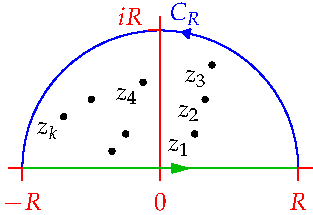
\includegraphics[scale=0.95]{integral}
\end{minipage}
\begin{enumerate}\setcounter{enumi}{2}
  \item If $\displaystyle\lim\limits_{R\to\infty}\int_{C_R}f(z)\,\dz=0$, then
$\displaystyle\text{P.V.}\int_{-\infty}^\infty f(x)\,\dx
=2\pi i\sum\limits_{k=1}^n\Resl{z=z_k}f(z)$
\end{enumerate}

The method is easiest when applied to rational functions $f(z)=\frac{p(z)}{q(z)}$, though it works more generally. Beyond the relative ease of residue calculation, one reason to stick to rational functions is that $\deg q\ge \deg p+2$ is enough to guarantee convergence in step 3 (Exercise \ref{exs:rationalimpint}).

\goodbreak


\begin{examples}{}{impexs}
	\exstart $f(z)=\frac 1{z^2+1}=\frac 1{(z-i)(z+i)}$ has simple poles at $\pm i$. Provided $\nm z=R>1$,
	\begin{enumerate}\setcounter{enumi}{1}
	  \begin{minipage}[t]{0.65\linewidth}\vspace{-10pt}
	  \item[]\begin{gather*}
		  \nm{z^2+1}\ge \nm{\nm z^2-1}=R^2-1
		  \implies\frac 1{\nm{z^2+1}}\le\frac 1{R^2-1}\\
		  \implies\nm{\oint_{C_R}f(z)\,\dz}\le \frac{\pi R}{R^2-1}\xrightarrow[R\to\infty]{}0\\
		  \implies \,\text{P.V.}\int_{-\infty}^\infty\frac 1{x^2+1}\,\dx
		  	=2\pi i\Resl{z=i}f(z)=\frac{2\pi i}{2i}=\pi
	  \end{gather*}
	  Compare with the usual calculus method:
	  \[
	  	\int_{-\infty}^\infty \frac 1{x^2+1}\,\dx=\tan^{-1}x\Big|_{-R_1\to-\infty}^{R_2\to\infty}=\pi
	  \]
		\end{minipage}
		\hfill
		\begin{minipage}[t]{0.34\linewidth}\vspace{0pt}
			\flushright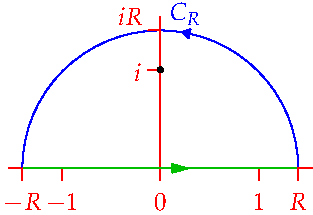
\includegraphics[scale=0.95]{integral2}
		\end{minipage}\smallbreak
	  
	  
	  \begin{minipage}[t]{0.65\linewidth}\vspace{0pt}
			\item $f(z)=\frac{4(z^2-1)}{z^4+16}$ has simple poles at $\pm 2\zeta,\pm 2\zeta^3$ where $\zeta=\polar{\pi i}4$.\par
			Let $p(z)=16(z^2-1)$ and $q(z)=z^4+16$, so that
		  \[
		  	\Res\limits_{z=z_0}f(z)=\frac{p(z_0)}{q'(z_0)}=\frac{z_0^2-1}{z_0^3}
		  \]
			When $\nm z=R>2$, we see that
		\end{minipage}
		\hfill
		\begin{minipage}[t]{0.34\linewidth}\vspace{0pt}
			\flushright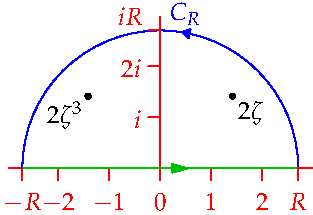
\includegraphics[scale=0.95]{integral3}
		\end{minipage}\par\vspace{-5pt}
	  \begin{gather*}
		  \nm{z^4+16}\ge R^4-16
		  	\implies \nm{\oint_{C_R}f(z)\,\dz}
		  	\le\frac{4\pi R(R^2+1)}{R^4-16}\to 0\\
		  \text{P.V.\ }\int_{-\infty}^\infty f(x)\,\dx 
		  	=2\pi i\left(\Resl{z=2\zeta}f(z)+\Resl{z=2\zeta^3}f(z)\right) 
		  	=2\pi i\left(\frac{4\zeta^2-1}{8\zeta^3}+\frac{4\zeta^6-1}{8\zeta^9}\right) 
		  	=\frac{3\pi}{2\sqrt 2}%\\
		  %&=\frac{2\pi i}\zeta\left(\frac 48-\frac 1{8i}+\frac 4{8i}-\frac 18\right) =\frac{2\pi i\sqrt 2}{1+i}\cdot \frac 38(1-i) =\frac{3\pi}{2\sqrt 2}
	  \end{gather*}
	  
	
	  \item\label{ex:smallarc} Variations are possible, for instance by taking only part of a semi-circular arc. The function $f(z)=\frac 1{z^5+1}$ has five simple poles: the fifth-roots of $-1$.\par
	 	\begin{minipage}[t]{0.65\linewidth}\vspace{-10pt}
			Since the pole $\zeta\omega^2=-1$ lies on the negative real axis, the integral $\int_{-\infty}^\infty f(x)\,\dx$ diverges. Instead consider the arcs in the picture when $R>1$. Parametrizing $C_2$ via $z(t)=t\omega$,
			\begin{align*}
				\int_{\textcolor{purple}{C_2}}\frac 1{z^5+1}\,\dz
				&=\int_R^0\frac{\omega}{t^5+1}\,\dt
					=-\omega\int_0^R\frac{1}{t^5+1}\,\dt\\
				&=-\omega\int_{\textcolor{Green}{C_1}}\frac 1{z^5+1}\,\dz
			\end{align*}
		\end{minipage}
		\hfill
		\begin{minipage}[t]{0.34\linewidth}\vspace{-25pt}
			\flushright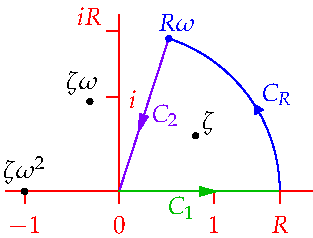
\includegraphics[scale=0.95]{integral4}
		\end{minipage}\par\vspace{-5pt}
		\[
			\implies(1-\omega)\int_0^R\frac 1{x^5+1}\,\dx
			+\int_{\textcolor{blue}{C_R}}\frac 1{z^5+1}\,\dz
			=2\pi i\Res_{z=\zeta}\frac 1{z^5+1} 
			=\frac{2\pi i}{5\zeta^4}
			=\frac{2\pi i}{5\omega^2}
		\]
		When $\nm z=R>1$, we see that $\smash[b]{\nm{z^5+1}\ge R^5-1\implies\nm{\int_{C_R}\frac 1{z^5+1}\,\dz}\le\frac{2\pi R}{5(R^5-1)}\xrightarrow[R\to\infty]{}0}$, and we conclude
		\[
			\int_0^\infty\frac 1{x^5+1}\,\dx
			=\frac{2\pi i}{5(\omega^2-\omega^3)} 
			=\frac{2\pi i}{5\zeta\omega^2(\zeta^{-1}-\zeta)} 
			=\frac{2\pi i}{5(2i\sin\frac\pi 5)}
			=\frac \pi 5\csc\frac\pi 5
		\]
	\end{enumerate}
\end{examples}


\goodbreak


\boldsubsubsection{Jordan's Lemma}

It is often desired, particularly when computing Fourier transforms,\footnote{%
	The Fourier transform of $f(x)$ is the function $\hat f(\xi):=\int_{-\infty}^\infty f(x)e^{-2\pi ix\xi}\,\dx$.%
} to evaluate integrals of the form
\[
	\int_{-\infty}^\infty f(x)e^{i ax}\,\dx
	=\int_{-\infty}^\infty f(x)\cos ax\,\dx
	+i\int_{-\infty}^\infty f(x)\sin ax\,\dx
\]
where $a>0$ is a real constant and $f:\R\to\C$ is a given function. If $f(x)$ is real-valued, then the above breaks the integral into real and imaginary parts. Given reasonable conditions on $f(x)$, the principal-value method can often be employed.

\begin{example}{}{}
	The function $f(z)=\frac{e^{3iz}}{z^2+4}$ is analytic on the upper half-plane except at the simple pole $z=2i$. With $R>2$ and $C_R$ the usual semi-circle, we see that
	\begin{gather*}
		\nm{e^{3iz}}=e^{-3y}\le 1
		\implies \nm{\int_{C_R}f(z)e^{3iz}\,\dz}
		\le \frac{\pi R}{R^2-4}\xrightarrow[R\to\infty]{} 0\\
		\implies \text{P.V.}\int_{-\infty}^\infty \frac{e^{3ix}}{x^2+4}\,\dx 
		=\lim_{R\to\infty}\int_{-R}^R \frac{e^{3ix}}{x^2+4}\,\dx 
		=2\pi i\Res_{z=2i}\frac{e^{3iz}}{z^2+4} 
		=2\pi i\frac{e^{-6}}{4i} 
		=\frac 12\pi e^{-6}
	\end{gather*}
	Since this is real, we see that the result is in fact the integral $\int_{-\infty}^\infty \frac{\cos 3x}{x^2+4}\,\dx$. We don't need the Cauchy principal value here since the full improper integral converges. The corresponding imaginary integral is trivially zero since $\frac{\sin x}{x^2+1}$ is an odd function.
\end{example}

To assist with such computations, we state the following result without proof.

\begin{thm}{Jordan's Lemma}{}
	Let $a,R_0>0$ be given and suppose $f(z)$ is analytic at all points exterior to the semi-circle $C_{R_0}$ in the upper half-plane. Suppose also that
	\[
		\forall R>R_0,\ \exists M_R\text{ such that } \nm z=R\implies \nm{f(z)}\le M_R\text{ and }\lim_{R\to\infty}M_R=0
	\]
	Then $\lim\limits_{R\to\infty}\int_{C_R}f(z)e^{i az}\,\dz=0$. If $f(z)$ moreover satisfies the hypotheses of our method, then
	\[
		\text{P.V.}\int_{-\infty}^\infty f(x)e^{i ax}\,\dx
		=2\pi i\sum_{k=1}^n\Res_{z=z_k}f(z)e^{i az}
	\]
\end{thm}

\begin{example}{}{}
	If $f(x)=\frac{x+1}{x^2+9}$ and $R>3$, then
	\begin{gather*}
		\nm{f(z)}=\frac{\nm{z+2}}{\nm{z^2+9}}
		\le\frac{R+2}{R^2-9}
		=M_R\xrightarrow[R\to\infty]{}0\\
		\implies \text{P.V.}\int_{-\infty}^\infty\frac{(x+2)e^{i ax}}{x^2+9}\,\dx
		=2\pi i\Res_{z=3i}\frac{(z+2)e^{iaz}}{z^2+9}
		=\frac{2\pi i(2+3i)e^{-3a}}{6i} 
		=\frac{\pi(2+3i)}3e^{-3a}
	\end{gather*}
	By considering even and odd functions, etc., we can rewrite this as
	\[
		\int_0^\infty\frac{\cos ax}{x^2+9}\,\dx 
		=\frac{\pi}{6}e^{-3a}
		\qquad \int_0^\infty\frac{x\sin ax}{x^2+9}\,\dx 
		=\frac{\pi}{2}e^{-3a}
	\]
\end{example}


\goodbreak


\boldinline{Indented paths}

Another modification allows $f(z)$ to have a simple pole on the real axis.

\begin{lemm}[lower separated=false, sidebyside, sidebyside align=top seam, sidebyside gap=0pt, righthand width=0.3\linewidth]{}{simppoleint}
	Let $D$ be the disk $\nm{z-z_0}\le\epsilon$, let $\delta<\epsilon$, and let $C_\delta$ be the clockwise semi-circle pictured.
	\begin{enumerate}
	  \item If $\phi(z)$ is analytic on $D$, then $\lim\limits_{\delta\to 0}\int_{C_\delta}\phi(z)\,\dz=0$.
	  \item If $f(z)$ is analytic on $D\setminus\{z_0\}$ with a simple pole at $z_0$, then
	  \[
	  	\lim_{\delta\to 0}\int_{C_\delta}f(z)\,\dz=-\pi i\Res_{z=z_0}f(z)
	  \] 
	\end{enumerate}
	\tcblower
	\flushright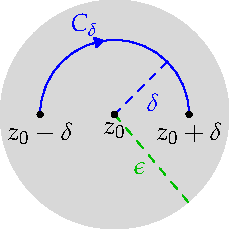
\includegraphics[scale=0.95]{integral5}
\end{lemm}

More generally, if $C_\delta$ spans $\theta$ radians clockwise round $z_0$, then $\lim\limits_{\delta\to 0}\int_{C_\delta}f(z)\,\dz=-i\theta\Res\limits_{z=z_0}f(z)$.

\begin{proof}
	\begin{enumerate}
	  \item $\phi$ is continuous on $D$ and is thus bounded by some $M$; but then $\nm{\int_{C_\delta}\phi(z)\,\dz}\le M\pi \delta$.
		\item The Laurent series expansion of $f(z)$ on $D\setminus\{z_0\}$ is
		\[
			f(z)=\frac{a_{-1}}{z-z_0}+\phi(z)
		\]
		where $a_{-1}=\Res\limits_{z=z_0}f(z)$ and $\phi(z)$ is analytic on $D$. Now observe that
		\[
			\int_{C_\delta}\frac{a_{-1}}{z-z_0}\,\dz=a_{-1}\int_{\pi}^0\frac 1{\delta e^{i\theta}}i\delta e^{i\theta}\,\dth =- ia_{-1}\int_{0}^\pi\,\dth=-\pi ia_{-1}
		\]
		is independent of $\delta$. By part (a), we conclude that $\lim\limits_{\delta\to 0}\int_{C_\delta}f(z)\,\dz=-\pi i\Res\limits_{z=z_0}f(z)$.\qedhere
	\end{enumerate}
\end{proof}

\begin{example}{}{}
	Consider $f(z)=\frac{e^{iz}}z$, which has a simple pole at $z_0=0$. If $0<\delta<R$, then
	\[
		\left(\textcolor{Green}{\int_{-R}^{-\delta}+\int_\delta^R}\right)f(x)\,\dx
		=\left(\int_{-R}^{-\delta}+\int_\delta^R\right)\frac{\cos x+i\sin x}{x}\,\dx
		=2i\int_\delta^R\frac{\sin x}x\,\dx
	\]
	
	\begin{minipage}[t]{0.59\linewidth}\vspace{0pt}
		by even/oddness. Moreover, by Lemma \ref{lemm:simppoleint},
		\[
			\lim_{\delta\to 0}\int_{C_\delta}\frac{e^{iz}}z\,\dz
			=-i\pi\Res_{z=0}f(z)=-i\pi
		\]
		Since $\nm{f(z)}=\frac{e^{-y}}R\le \frac 1R$ on $C_R$, Jordan's lemma tells us that
		\[
			0=2i\int_0^\infty\frac{\sin x}x\,\dx-i\pi
			\implies \int_0^\infty\frac{\sin x}x\,\dx=\frac\pi 2
		\]
	\end{minipage}
	\hfill
	\begin{minipage}[t]{0.4\linewidth}\vspace{0pt}
		\flushright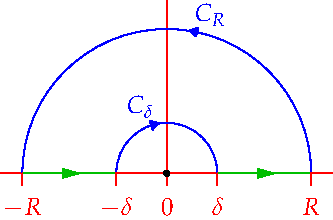
\includegraphics[scale=0.95]{integral6}
	\end{minipage}
\end{example}

The example relied on the evenness of $\frac{\sin x}x$ and on the fact that the region of the half-plane between $C_R$ and $C_\delta$ contains no poles of $f(z)$. We essentially evaluated $\int_0^R\frac{\sin x}x\,\dx=\frac 12\int_{-R}^R\frac{\sin x}x\,\dx$ using an \emph{indented path} lying on the $x$-axis but dodging round the simple pole at zero. Many other versions of this trick are possible!


\goodbreak


\begin{exercises}
	\hangindent\leftmargini
	Many of these problems require extensive calculations using residues. Take your time and use them as an excuse to practice.	
	\begin{enumerate}
	  \item Use residues to verify each improper integral:
	  \begin{enumerate}
	    \item \makebox[200pt][l]{$\displaystyle\int_0^\infty\frac{\dx}{(x^2+1)^2}=\frac\pi 4$\hfill (b) }\ 
	    $\displaystyle\int_0^\infty\frac{x^2\,\dx}{x^6+1}=\frac\pi 6$
	    \setcounter{enumii}{2}
	    \item \makebox[200pt][l]{$\displaystyle\int_0^\infty\frac{x^2\,\dx}{(x^2+1)(x^2+4)}=\frac\pi 6$ \hfill (d) }\
	    $\displaystyle\int_0^\infty\frac{x^2\,\dx}{(x^2+9)(x^2+4)^2}=\frac\pi{200}$
	  \end{enumerate}
	  
	  
	  \item Find the Cauchy principal value of each integral:
	  \begin{enumerate}
	    \item $\displaystyle\int_{-\infty}^\infty\frac{\dx}{x^2+2x+2}$
	    \qquad\qquad
	    (b)\ \ $\displaystyle\int_{-\infty}^\infty\frac{x\,\dx}{(x^2+1)(x^2+2x+2)}$
	  \end{enumerate}
	  
	  
	  \item Let $m,n$ be integers where $0\le m\le n-2$. By mimicking Example \ref*{ex:impexs}.\ref{ex:smallarc}, prove that
	  \[
	  	\int_0^\infty\frac{x^m}{x^n+1}\,\dx=\frac\pi n\csc\frac{(m+1)\pi}n
	  \]  
	 
	  
	  \item\begin{enumerate}
	    \item If $\int_{-\infty}^\infty f(x)\,\dx$ converges, prove that it equals its Cauchy principal value.
	    
	    \item Suppose $f(x)$ is an even function and that $\text{P.V.}\int_{-\infty}^\infty f(x)\,\dx$ exists. Prove that $\int_{-\infty}^\infty f(x)\,\dx$ exists and has the same value.
	  \end{enumerate}
	  
	  
	  \item\label{exs:rationalimpint} Suppose $f(x)=\frac{p(x)}{q(x)}$ is a rational function where $q(x)$ has no (real) zeros and $2+\deg p\le\deg q$. Prove that $\int_0^\infty f(x)\,\dx$ converges.\par
	  (\emph{Hint: let $p,q$ be monic and recall the comparison test for improper integrals})
	
	
	  \item Prove the identities:
	  \begin{enumerate}
	    \item $\displaystyle\int_{-\infty}^\infty \frac{\cos x\,\dx}{(x^2+a^2)(x^2+b^2)} =\frac\pi{a^2-b^2}\left(\frac{e^{-b}}b-\frac{e^{-a}}a\right)$ \ if $a>b>0$
	    
	    %\item $\displaystyle\int_{0}^\infty \frac{\cos ax\,\dx}{x^2+1} =\frac\pi 2e^{-a}$ if $a>0$
	    
	    \item $\displaystyle\int_{0}^\infty \frac{\cos ax\,\dx}{(x^2+b^2)^2} =\frac\pi{4b^3}(1+ab)e^{-ab}$ \ if $a,b>0$
	    
	    %\item $\displaystyle\int_{-\infty}^\infty \frac{x\sin ax\,\dx}{x^4+4} =\frac\pi 2e^{-a}\sin a$ if $a>0$
		\end{enumerate}
		
		
		\item Evaluate the integrals:
	  \begin{enumerate}
	    \item $\displaystyle\int_{-\infty}^\infty \frac{x\sin x\,\dx}{(x^2+1)(x^2+4)}$
	    \qquad\qquad
	    (b)\ \ $\displaystyle\int_{0}^\infty \frac{x^3\sin x\,\dx}{(x^2+1)(x^2+9)}$
		\end{enumerate}
		
		
		\item If $a$ is any real number and $b>0$, find the Cauchy principal value of $\displaystyle\int_{-\infty}^\infty\frac{\cos x\,\dx}{(x+a)^2+b^2}$
		
		
		\item Use $f(z)=z^{-2}(e^{i az}-e^{i bz})$ and an indented contour around $z_0=0$ to prove that
		\[
			\int_0^\infty \frac{\cos ax-\cos bx}{x^2} =\frac\pi 2(b-a)
			\quad\text{whenever}\quad
			a,b\ge 0
		\]
		
		
		\item By integrating $f(z)=\frac{z^{-1/2}}{z^2+1}=\frac{\exp(-\frac 12\log z)}{z^2+1}$ where $\arg z\in(-\frac\pi 2,\frac{3\pi}2)$ along an indented contour, prove that
		\[
			\int_0^\infty \frac{\dx}{\sqrt x(x^2+1)} =\frac\pi{\sqrt 2}
		\]
	  
	  
	  \item What happens to part 2 of Lemma \ref{lemm:simppoleint} if $f(z)$ is analytic on $D\setminus\{z_0\}$ but has a pole of order $m\ge 2$ at $z_0$.
	  
	  
		\item (Hard)\quad A similar trick can be applied with sequences of boundary curves $C_N$. For instance, for each $N\in\N$, let $C_N$ denote the positively oriented boundary of the square whose edges lie along the lines $x,y=\pm\left(N+\frac 12\right)\pi$. Prove that
	  \[
	  	\oint_{C_N}\frac{\dz}{z^2\sin z}=2\pi i\left[\frac 16+2\sum_{n=1}^N\frac{(-1)^n}{n^2\pi^2}\right]
	  \]
	  Hence conclude that $\sum\limits_{n=1}^\infty\frac{(-1)^{n-1}}{n^2}=\frac{\pi^2}{12}$, and $\sum\limits_{n=1}^\infty\frac{1}{n^2}=\frac{\pi^2}{6}$.
	\end{enumerate}
\end{exercises}
